
\begin{frame}{WTS methods}
    \begin{columns}
        \begin{column}{0.6\textwidth}
            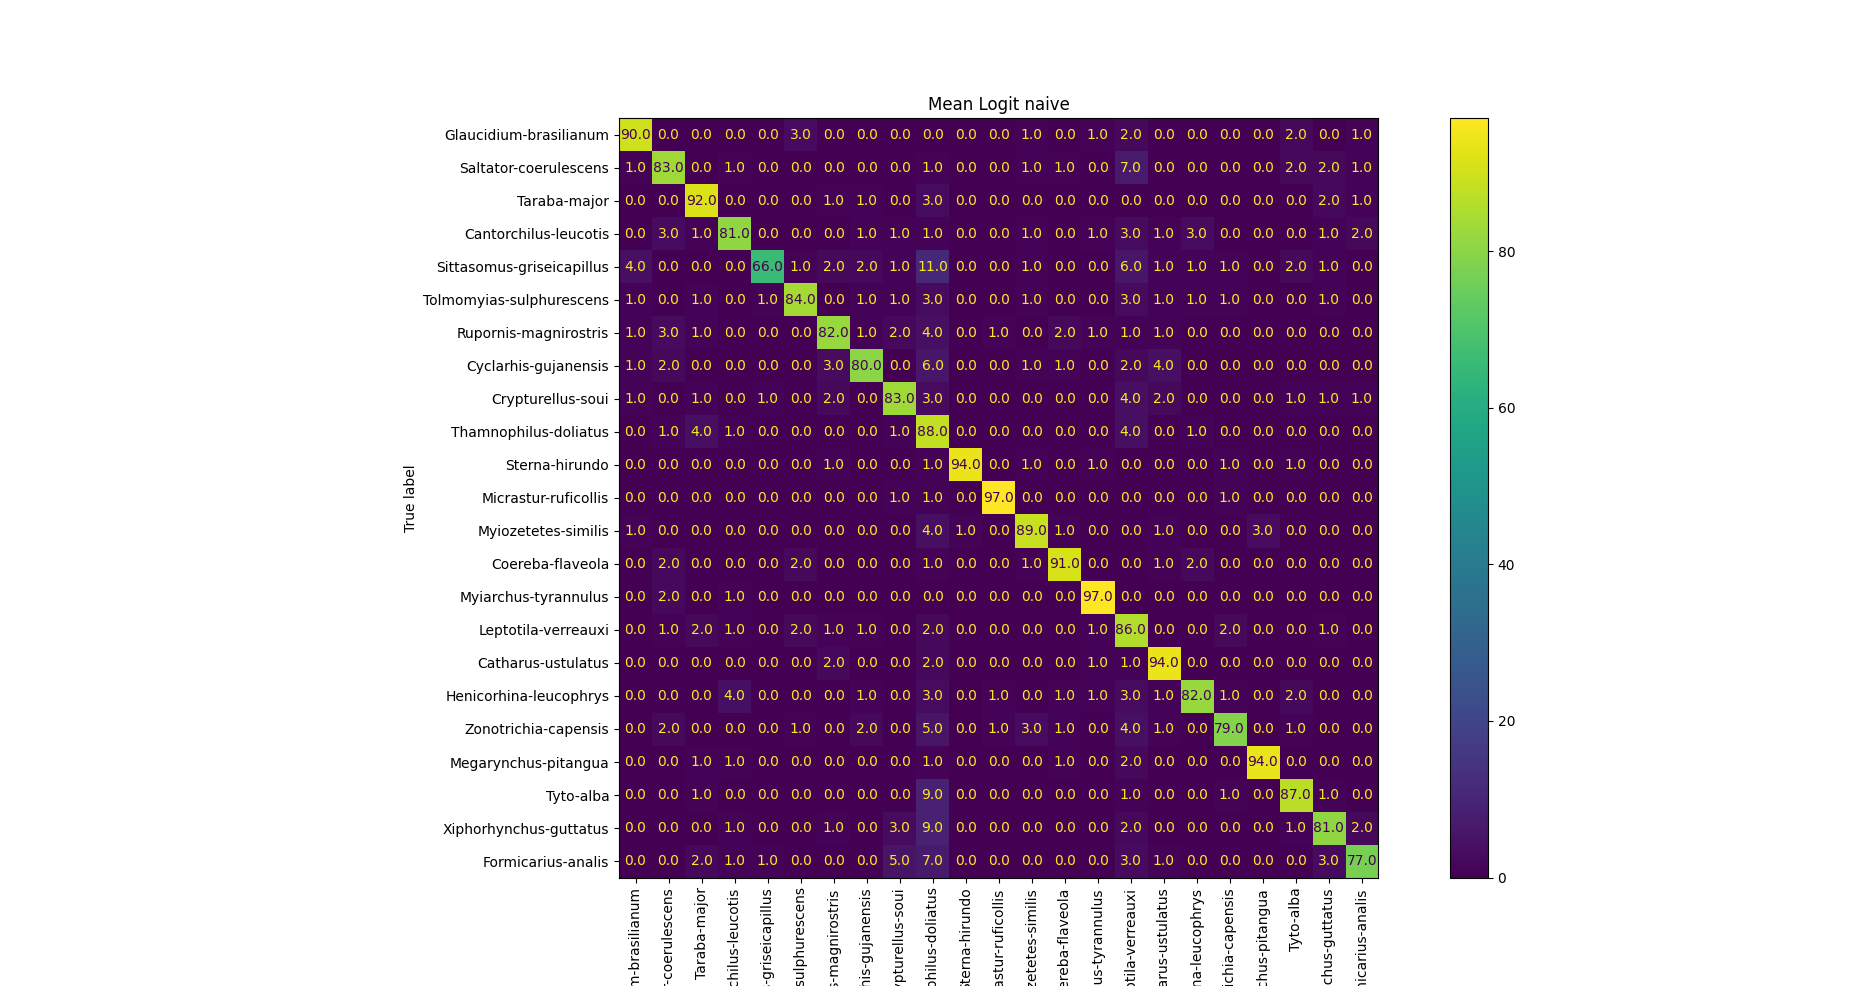
\includegraphics[height=0.7\textheight,width=0.7\textwidth,keepaspectratio]{images/conf_mat_naive.png}
            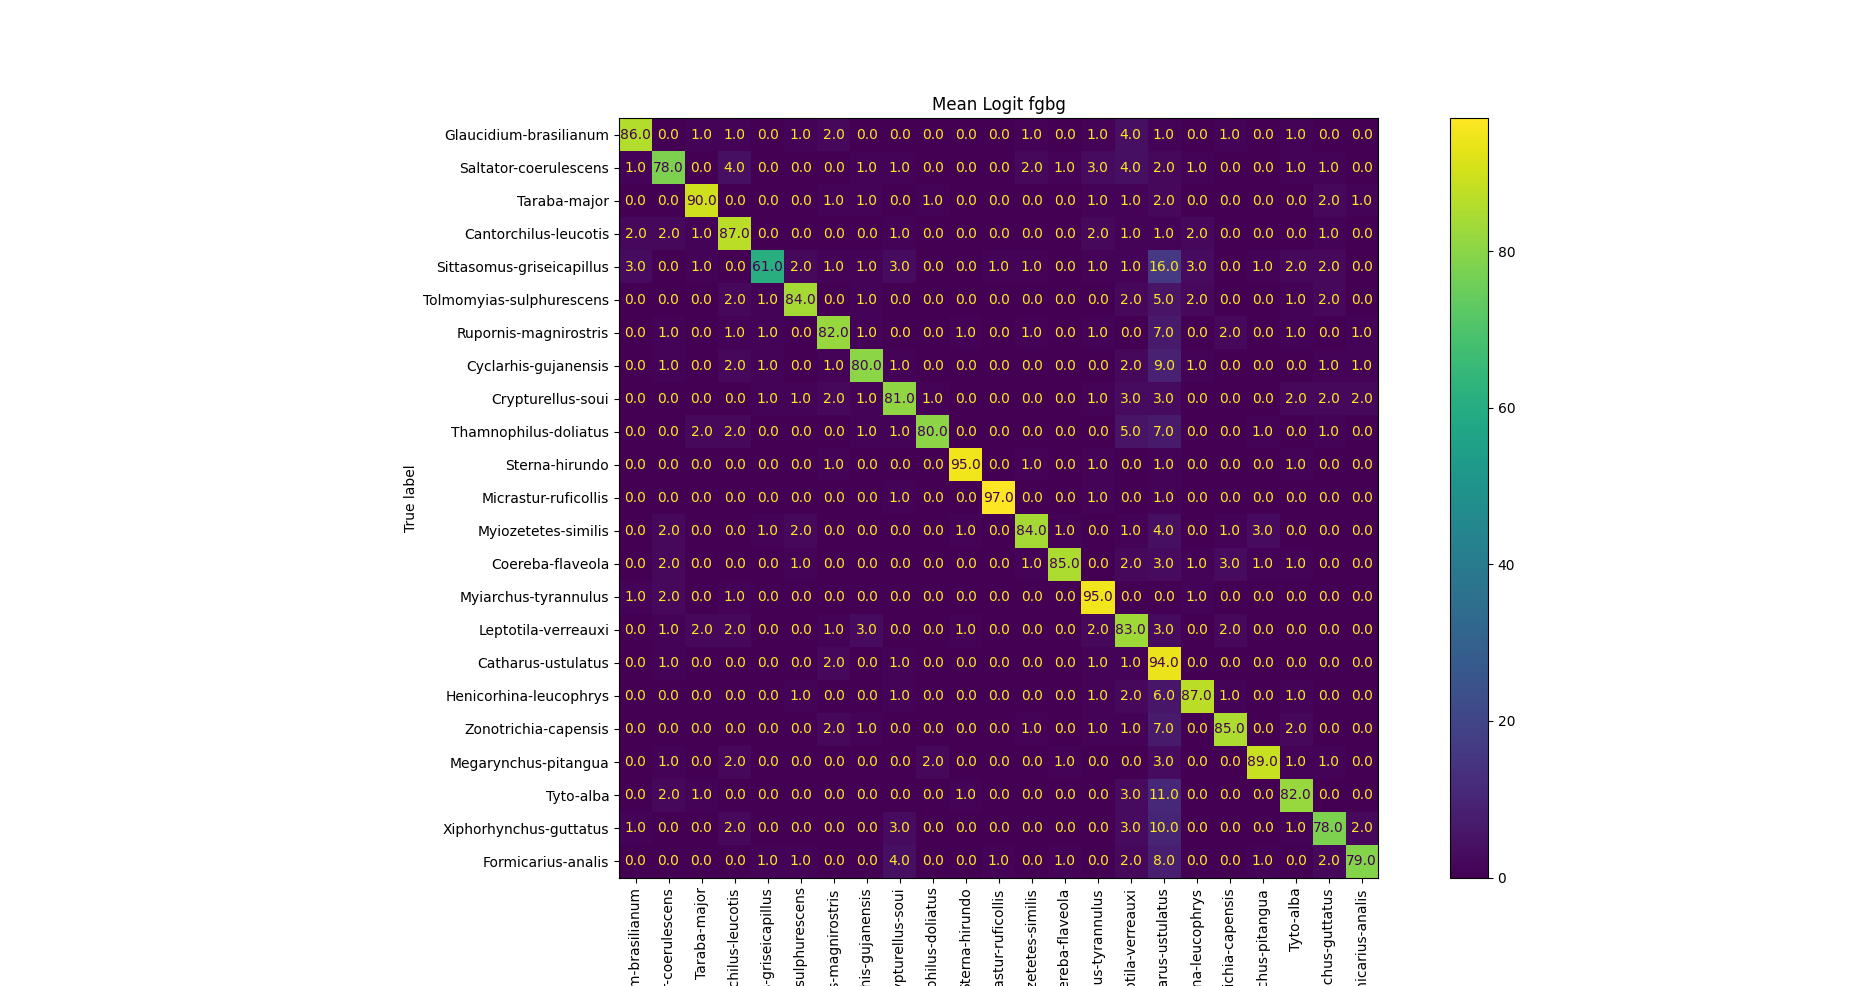
\includegraphics[height=0.7\textheight,width=0.7\textwidth,keepaspectratio]{images/conf_mat_fgbg.png}
        \end{column}
        \begin{column}{0.6\textwidth}
            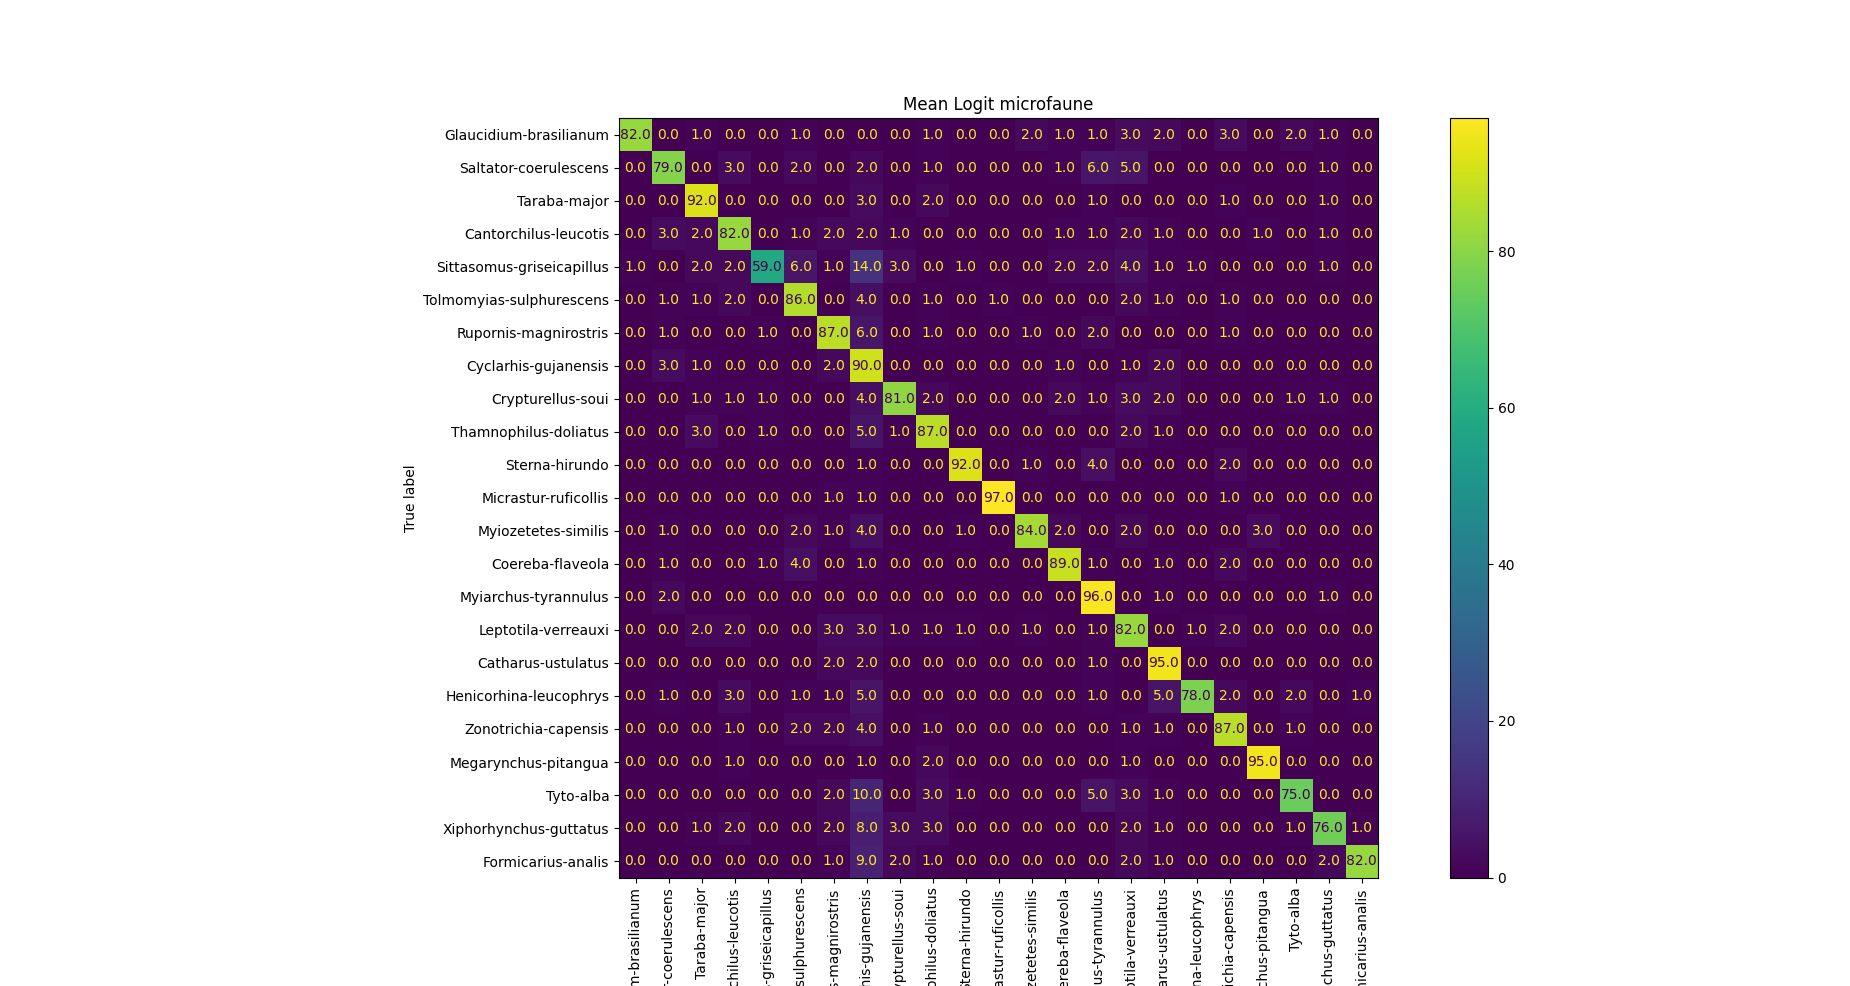
\includegraphics[height=0.7\textheight,width=0.7\textwidth,keepaspectratio]{images/conf_mat_microfaune.png}
            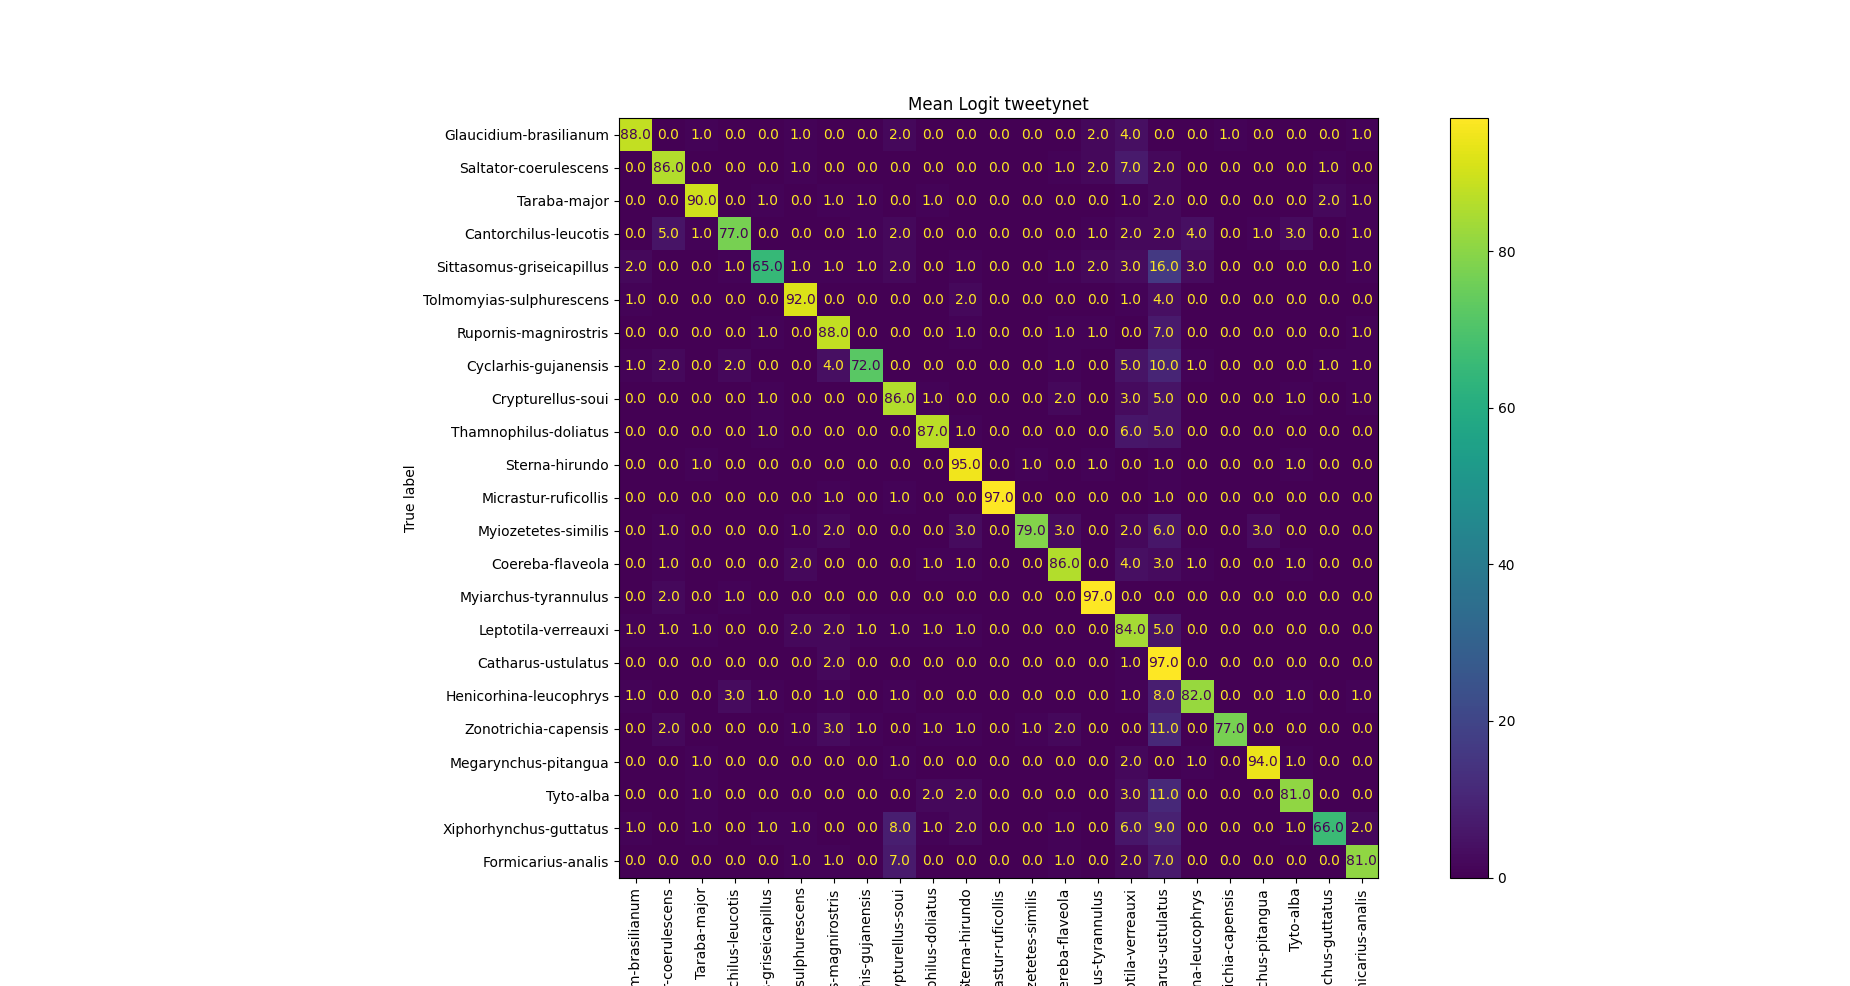
\includegraphics[height=0.7\textheight,width=0.7\textwidth,keepaspectratio]{images/conf_mat_tweetynet.png}
        \end{column}
    \end{columns}
\end{frame}

\begin{frame}{Deep Learning Template Matching Verification}
    \centering
    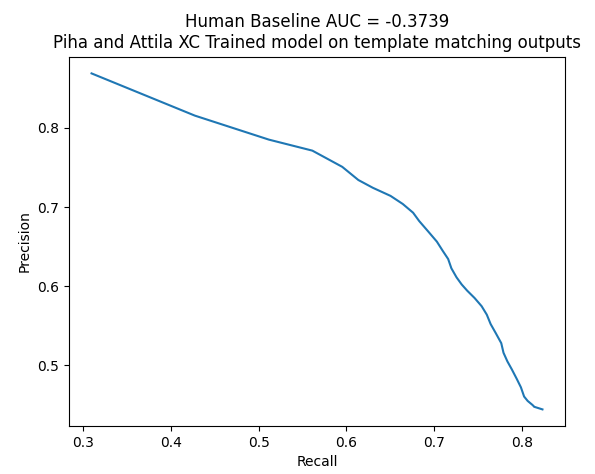
\includegraphics[height=0.7\textheight,width=0.7\textwidth,keepaspectratio]{images/TMV-precision-recall.png}
    \begin{itemize}
        \item 70\% CMAP
        \item songs, not chirps
    \end{itemize}
\end{frame}

\begin{frame}{Download this For Later}
    \begin{itemize}
        \item \url{https://drive.google.com/file/d/1E-e2tlg8GpQ3M4pIR-pRh1L9ZY4ROfgI/view?usp=sharing}
    \end{itemize}
\end{frame}

\begin{frame}{GradCam}
    \centering
    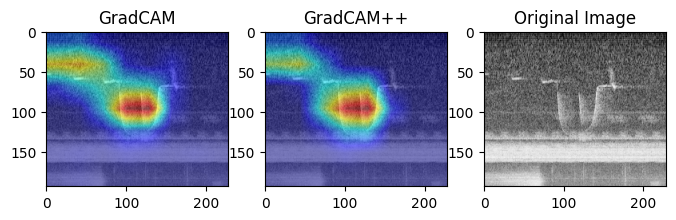
\includegraphics[height=0.7\textheight,width=0.7\textwidth,keepaspectratio]{./images/screaming_gradcam_1.png}

\end{frame}
\begin{frame}{GradCam Math}
    \centering
    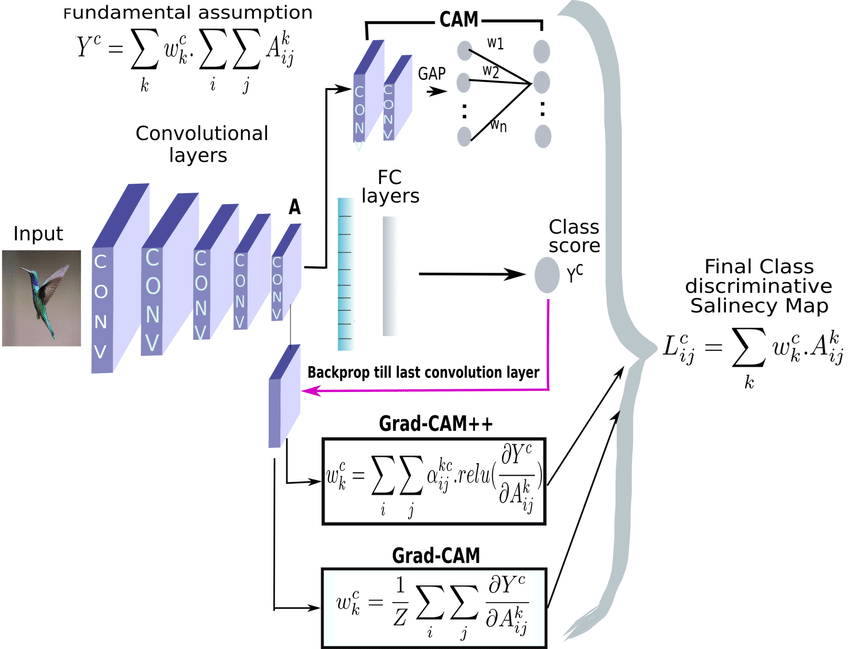
\includegraphics[height=0.7\textheight,width=0.7\textwidth,keepaspectratio]{./images/grad_cam_explination.png}

    Grad-CAM++: Generalized Gradient-based Visual Explanations for Deep Convolutional Networks
\end{frame}
\begin{frame}{GradCam++ Evaluation}
    \begin{itemize}
        \item Subjective (Human trust)
        \item \url{https://drive.google.com/file/d/1E-e2tlg8GpQ3M4pIR-pRh1L9ZY4ROfgI/view?usp=sharing}
        \item Objective (Drop in Confidence)
    \end{itemize}
\end{frame}
\begin{frame}{GradCam++ Evaluation}
    \centering
    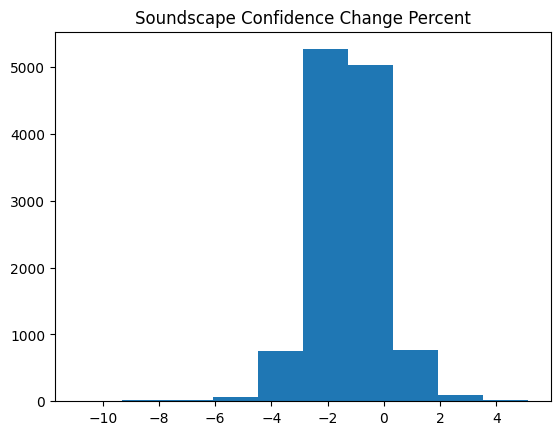
\includegraphics[height=0.7\textheight,width=0.7\textwidth,keepaspectratio]{./images/Soundscape_Confidence.png}
\end{frame}
\begin{frame}{GradCam++ Evaluation}
    \centering
    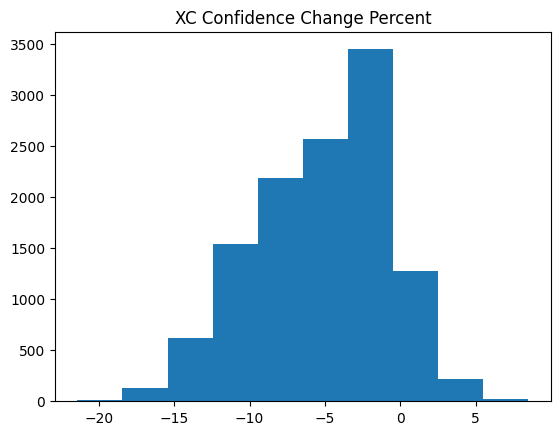
\includegraphics[height=0.7\textheight,width=0.7\textwidth,keepaspectratio]{./images/XC_conf.png}
\end{frame}
\begin{frame}{GradCam Bottom Line}
    \begin{itemize}
        \item The activation maps, look good
        \item confidence drops seem reasonable
        \item Hypothesis: the model is able to pick out useful features in spectrograms
    \end{itemize}
\end{frame}


\begin{frame}{Looking at everything}
    \begin{itemize}
        \item For XC models:
        \item Jacob: Good if testing against songs
        \item Sean: Find useful features in soundcapes
        \item OVERALL:
        \item The models might be decent
        \item The test data may not test the problem
    \end{itemize}
\end{frame}



% Slides for 2024-04-29
% To create a slide, use the following:
% \begin{frame}{TITLE}
%     BODY
% \end{frame}

% To create a slide with a bullet list, use the following:
% \begin{frame}{TITLE}
%     \begin{itemize}
%         \item ITEM 1
%         \item ITEM 2
%     \end{itemize}    
% \end{frame}

% To create a slide with numbered list, use the following:
% \begin{frame}{TITLE}
%     \begin{enumerate}
%         \item ITEM 1
%         \item ITEM 2
%     \end{enumerate}
% \end{frame}

% To create a slide with a graphic:
% 1. Add the graphic to this folder (named picture.png)
% 2. Use the following:
% \begin{frame}{TITLE}
%     \centering
%     \includegraphics[height=0.7\textheight,width=0.7\textwidth,keepaspectratio]{picture.png}
% \end{frame}

% To create a slide with two columns, use the following:
% \begin{frame}{TITLE}
%     \begin{columns}
%         \begin{column}{0.5\textwidth}
%             COLUMN 1 BODY
%         \end{column}
%         \begin{column}{0.5\textwidth}
%             COLUMN 2 BODY
%         \end{column}
%     \end{columns}
% \end{frame}

